% !TEX root = ../../main.tex

\section{Shaping in context}

In order to understand the requirement for material forming, 
we should first examine adsorption from 
a kinetic and thermal standpoint. 
Until now, in this thesis the isotherms were measured in systems
that achieved complete equilibrium between each step, without 
a mention of experimental duration. However, this parameter is crucial
when working with time-dependent systems operating in a
flow mode, as columns and beds rarely operate at equilibrium
conditions.

The rate of adsorption on the surface of the pore is theoretically 
immediate, with the controlling step being diffusion of guest
molecules between particles (interparticle) and through the pore network 
(intraparticle)~\cite{ruthvenPressureSwingAdsorption1994}.
Diffusion is dominated by different phenomena depending on the
lengthscale involved, from molecular diffusion or Knudsen diffusion
in large pores, to concentration gradients and steric effects in
micropores. Forced flow regimes dramatically improve interparticle
and particle surface diffusion at the cost of the energy required
to impose the pressure drop. A balance must be struck to obtain a 
high overall diffusion coefficient while maintaining a large surface 
area to volume ratio and a reasonable pressure drop across the 
column or bed~\cite{mitchellAdvancedVisualizationStrategies2013}.

As mentioned in \autoref{calo}, adsorption is an exothermic process,
with high amounts of heat released (corresponding to the integral 
enthalpy of adsorption \gls{dH}). Since rates and 
capacity are dictated by an Arrhenius-type law, an increase in temperature 
leads to lower capacities, and is rarely desired. 
As with diffusion, fast thermal transfer is therefore needed
to prevent a loss in efficiency or, with some materials, a degradation
of the adsorbent itself.

Finally, the mechanical resistance of the material used in a 
bed or column should be considered. The flow regime 
used to improve diffusion and heat transfer 
may lead to attrition and breakage of the 
adsorbent structure. Often in tall columns, the weight of the 
material itself can be a factor that leads to structural
collapse.

The requirements discussed above lead to the necessity of adsorbent
forming or shaping. The forming process generates a hierarchical pore size 
distribution which helps with reducing pressure drop, as can be
seen in \autoref{shaping:fig:particle}. The addition of 
binders or other additives improves the mechanical and thermal
properties of the final shaped material. Depending on the application,
many types of shaped materials exist, from simple granules and 
pellets, to rods, monoliths and membranes.
The process itself consists of extrusion of the particle-binder slurry 
and then hardening either through temperature, cross-linking
or chemical treatment. Other methods, such as spray-drying or 
granulation can similarly be 
used~\cite{ruthvenPrinciplesAdsorptionAdsorption1984}.
While the basic steps are the same: mixing the powder with
additives, shaping in the required form and curing of the final
structure, many variations are possible in each step.

\begin{figure}[!htb]
	\centering
	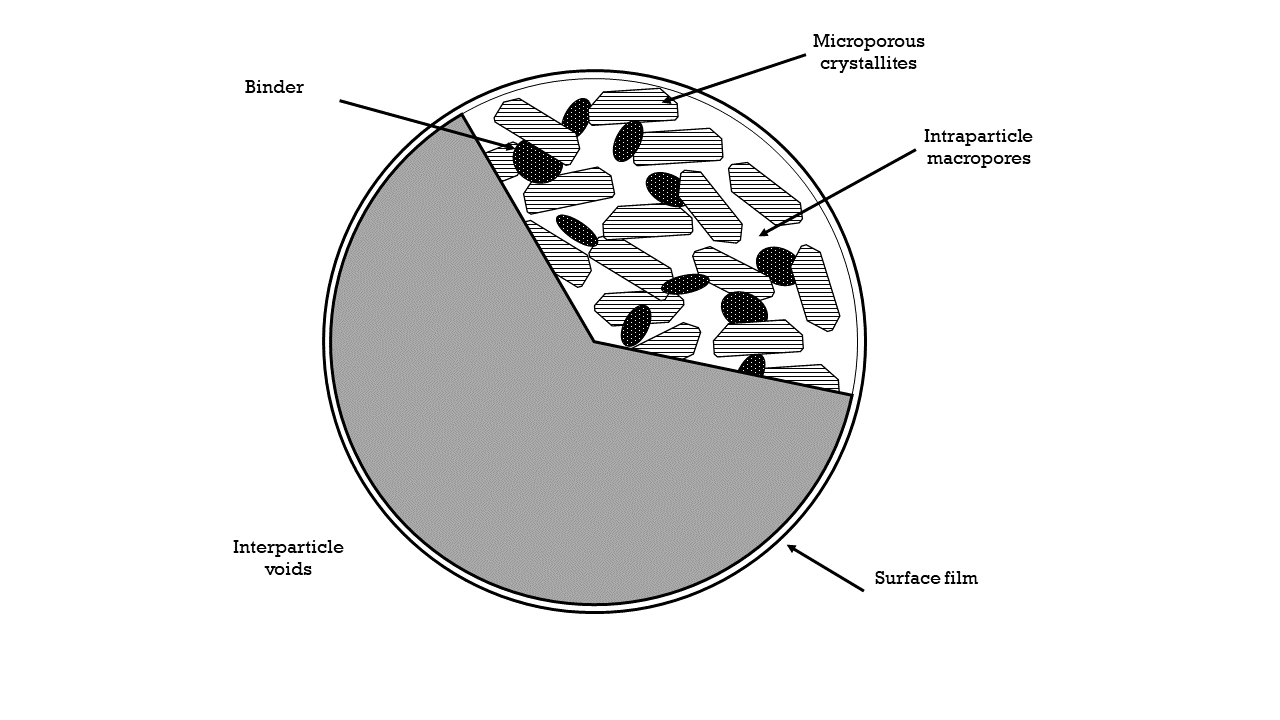
\includegraphics[width=0.8\textwidth]{shapedparticle}
	\caption{An schematic representation of the possible structure
	of a shaped sphere.}%
	\label{shaping:fig:particle}
\end{figure}

The binders, as their name imply, serve to hold crystals together
during and after the shaping process.
For carbons, binders such as pitch, polymers (CMC, \gls{PVA}) or 
even non-porous carbon black are 
commonly used~\cite{ohjiAdvancedProcessingManufacturing2008}.
For zeolites, inorganic binders are more prevalent, with silica, 
alumina and clay binders common in industry. 
Often, a combination of additives is used, each with a different role 
during the pelletization process~\cite{bandoszActivatedCarbonSurfaces2006}
such as improving rheological behaviour. It has been 
shown~\cite{whitingcuriouscasezeolite2016, MichelsEffectsBindersPerformance2014}
that the choice of binder can introduce large property variations, ranging 
from loss of porosity and structure to the enhancement of the desired
reactivity and selectivity through changes in the acid site density 
or ion migration.

Overall, during shaping the capacity per mass of pellet is expected to 
decrease due to the addition of a non-porous component, but the
difference should be small and should not arise due to effects 
such as pore blocking or pore filling with the binder material.
Furthermore, a densification is expected as the low density bulk powder
is compressed in the final material, leading to
better performance on a volume basis.
Finally, binder addition should not influence the chemical properties 
of the adsorbent, and preserve the original interactions with the adsorptives.
With a judicious choice of binding material, the resulting pellet
may even outperform the powder.

When it comes to \glspl{MOF}, shaping has been attempted with a wide range
of binders and methods. 
Methods such as granulation, spray-drying or extrusion have
all been successfully employed to create \gls{MOF}
pellets~\cite{kaskelChemistryMetalorganicFrameworks2016}.
Monoliths have also been shown to be an effective way for shaping purposes,
either through impregnation~\cite{ramos-fernandezMOFsMeetMonoliths2011} 
or through support on alumina~\cite{aguadoFacileShapingImidazolatebased2010}.
Surprisingly, compression~\cite{bazer-bachiIndustrialUseMetalorganic2014} or
even simple air drying of \gls{MOF} 
slurries~\cite{tianMechanicallyChemicallyRobust2015}
have also shown good results. Note that the monolith prepared 
through the latter method had a three times larger volumetric 
specific surface area than the conventional powder.

The connection between \gls{MOF} and binder is also of crucial importance. 
The \gls{MOF}-polymer interface has been 
shown~\cite{seminoMicroscopicModelMetal2016} to be
subject to a complex interplay of interactions between the organic
chains and the crystal surfaces. These effects can be striking enough 
to warrant further research into \gls{MOF}-polymer 
hybrids~\cite{kitaoHybridizationMOFsPolymers2017}, with the aim 
of combining the unique attributes of both materials.

Previous work from MADIREL~\cite{chanutObservingEffectsShaping2016} 
has analysed the impact of \gls{PVA} shaping on a series 
of \glspl{MOF}. It was shown that the binder did introduce some specific 
effects, such as a protection effect on the reduction of \ce{Fe^3+} to
\ce{Fe^2+} in MIL-127(Fe), as well as a curious gateing effect seen on 
butane adsorption on MIL-100(Fe), likely due to polymer chains covering 
pore entrances. Otherwise, the shaping imparted good performance to the
shaped samples, with almost no capacity loss on
a mass basis. Unfortunately, the use of a polymer limited the 
activation temperature of the samples to a maximum of 
\SI{150}{\degreeCelsius}.